\documentclass{article}
\usepackage[utf8]{inputenc}
\usepackage[utf8]{inputenc}
\usepackage{bigints}
\usepackage{graphicx}
\usepackage[left=35mm,top=26mm,right=25mm,bottom=15mm]{geometry}
\usepackage{amsmath}
\usepackage{array}

\title{\Huge \textbf{AE 238 Assignment 1}}
\author{\Huge \textbf{Krishna Wadhwani - 160010031 }}
\date{January 2018}

\begin{document}

\maketitle

%\title{\textbf{ \LARGE Question 1}}
\begin{center}
\title{\textbf{\underline{ \LARGE Question 1}}}
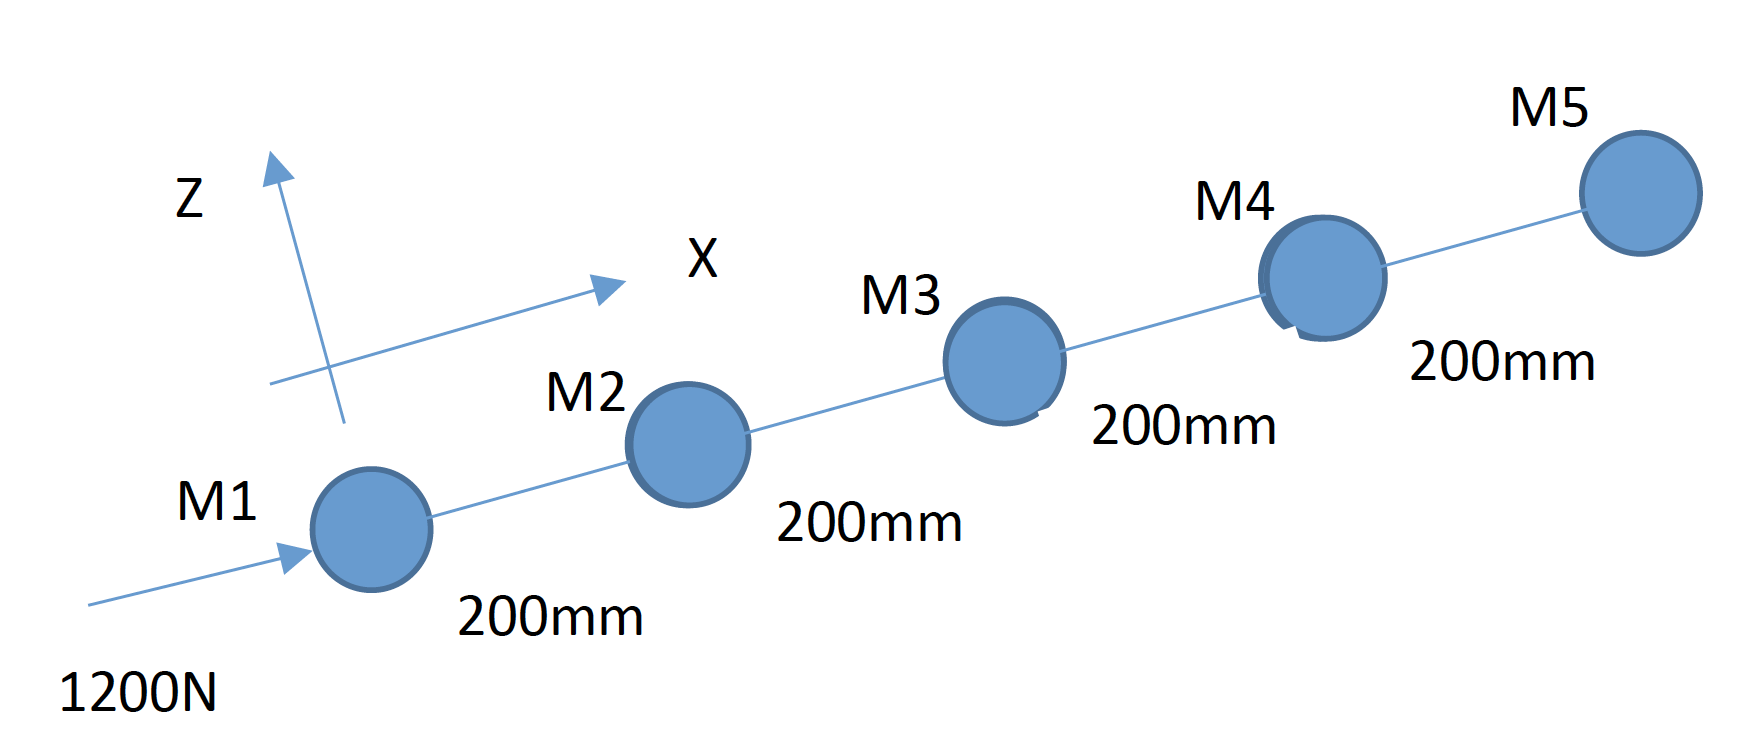
\includegraphics[scale=0.4]{238Q1.png}
\end{center}

NOTE: \begin{itemize}
    \item $W_{Ai}$ denotes apparant weight of the ith body (body with mass $M_i$).
    \item $R_{i,cg}$ denotes \underline{distance} of the ith body from the centre of gravity
    \item Value of $g$ is taken as $10\ m/s^2$
    \item Anti-clockwise moment is considered positive
\end{itemize}
Given: \\

\begin{tabular}{ | m{1cm} | m{1cm}|} 
\hline
$M_1$ & 50 kg  \\ 
\hline
$M_2$ & 200 kg  \\  
\hline
$M_3$ & 100 kg \\ 
\hline
$M_4$ & 100 kg  \\ 
\hline
$M_5$ & 50 kg\\
\hline
\end{tabular}
\bigbreak

\noindent Finding position of centre of gravity: \\

\noindent $x_{cg}= \sum_{i=1}^5 M_ix_i$\\
$x_{cg}=\dfrac{M_1 \times 0 + M_2 \times 200 + M_3 \times 400 + M_4 \times 600 + M_5 \times 800}{5}$\\
$x_{cg}= 360\ mm$\\

\begin{tabular}{ | m{1cm} | m{1cm}|} 
\hline
$R_{1cg}$ & 0.36 m  \\ 
\hline
$R_{2cg}$ & 0.16m  \\  
\hline
$R_{3cg}$ & 0.04 m \\ 
\hline
$R_{4cg}$ & 0.24 m  \\ 
\hline
$R_{5cg}$ & 0.44 m\\
\hline
\end{tabular}
\bigbreak

\noindent \underline{Analyzing Mass $M_1$}:\\

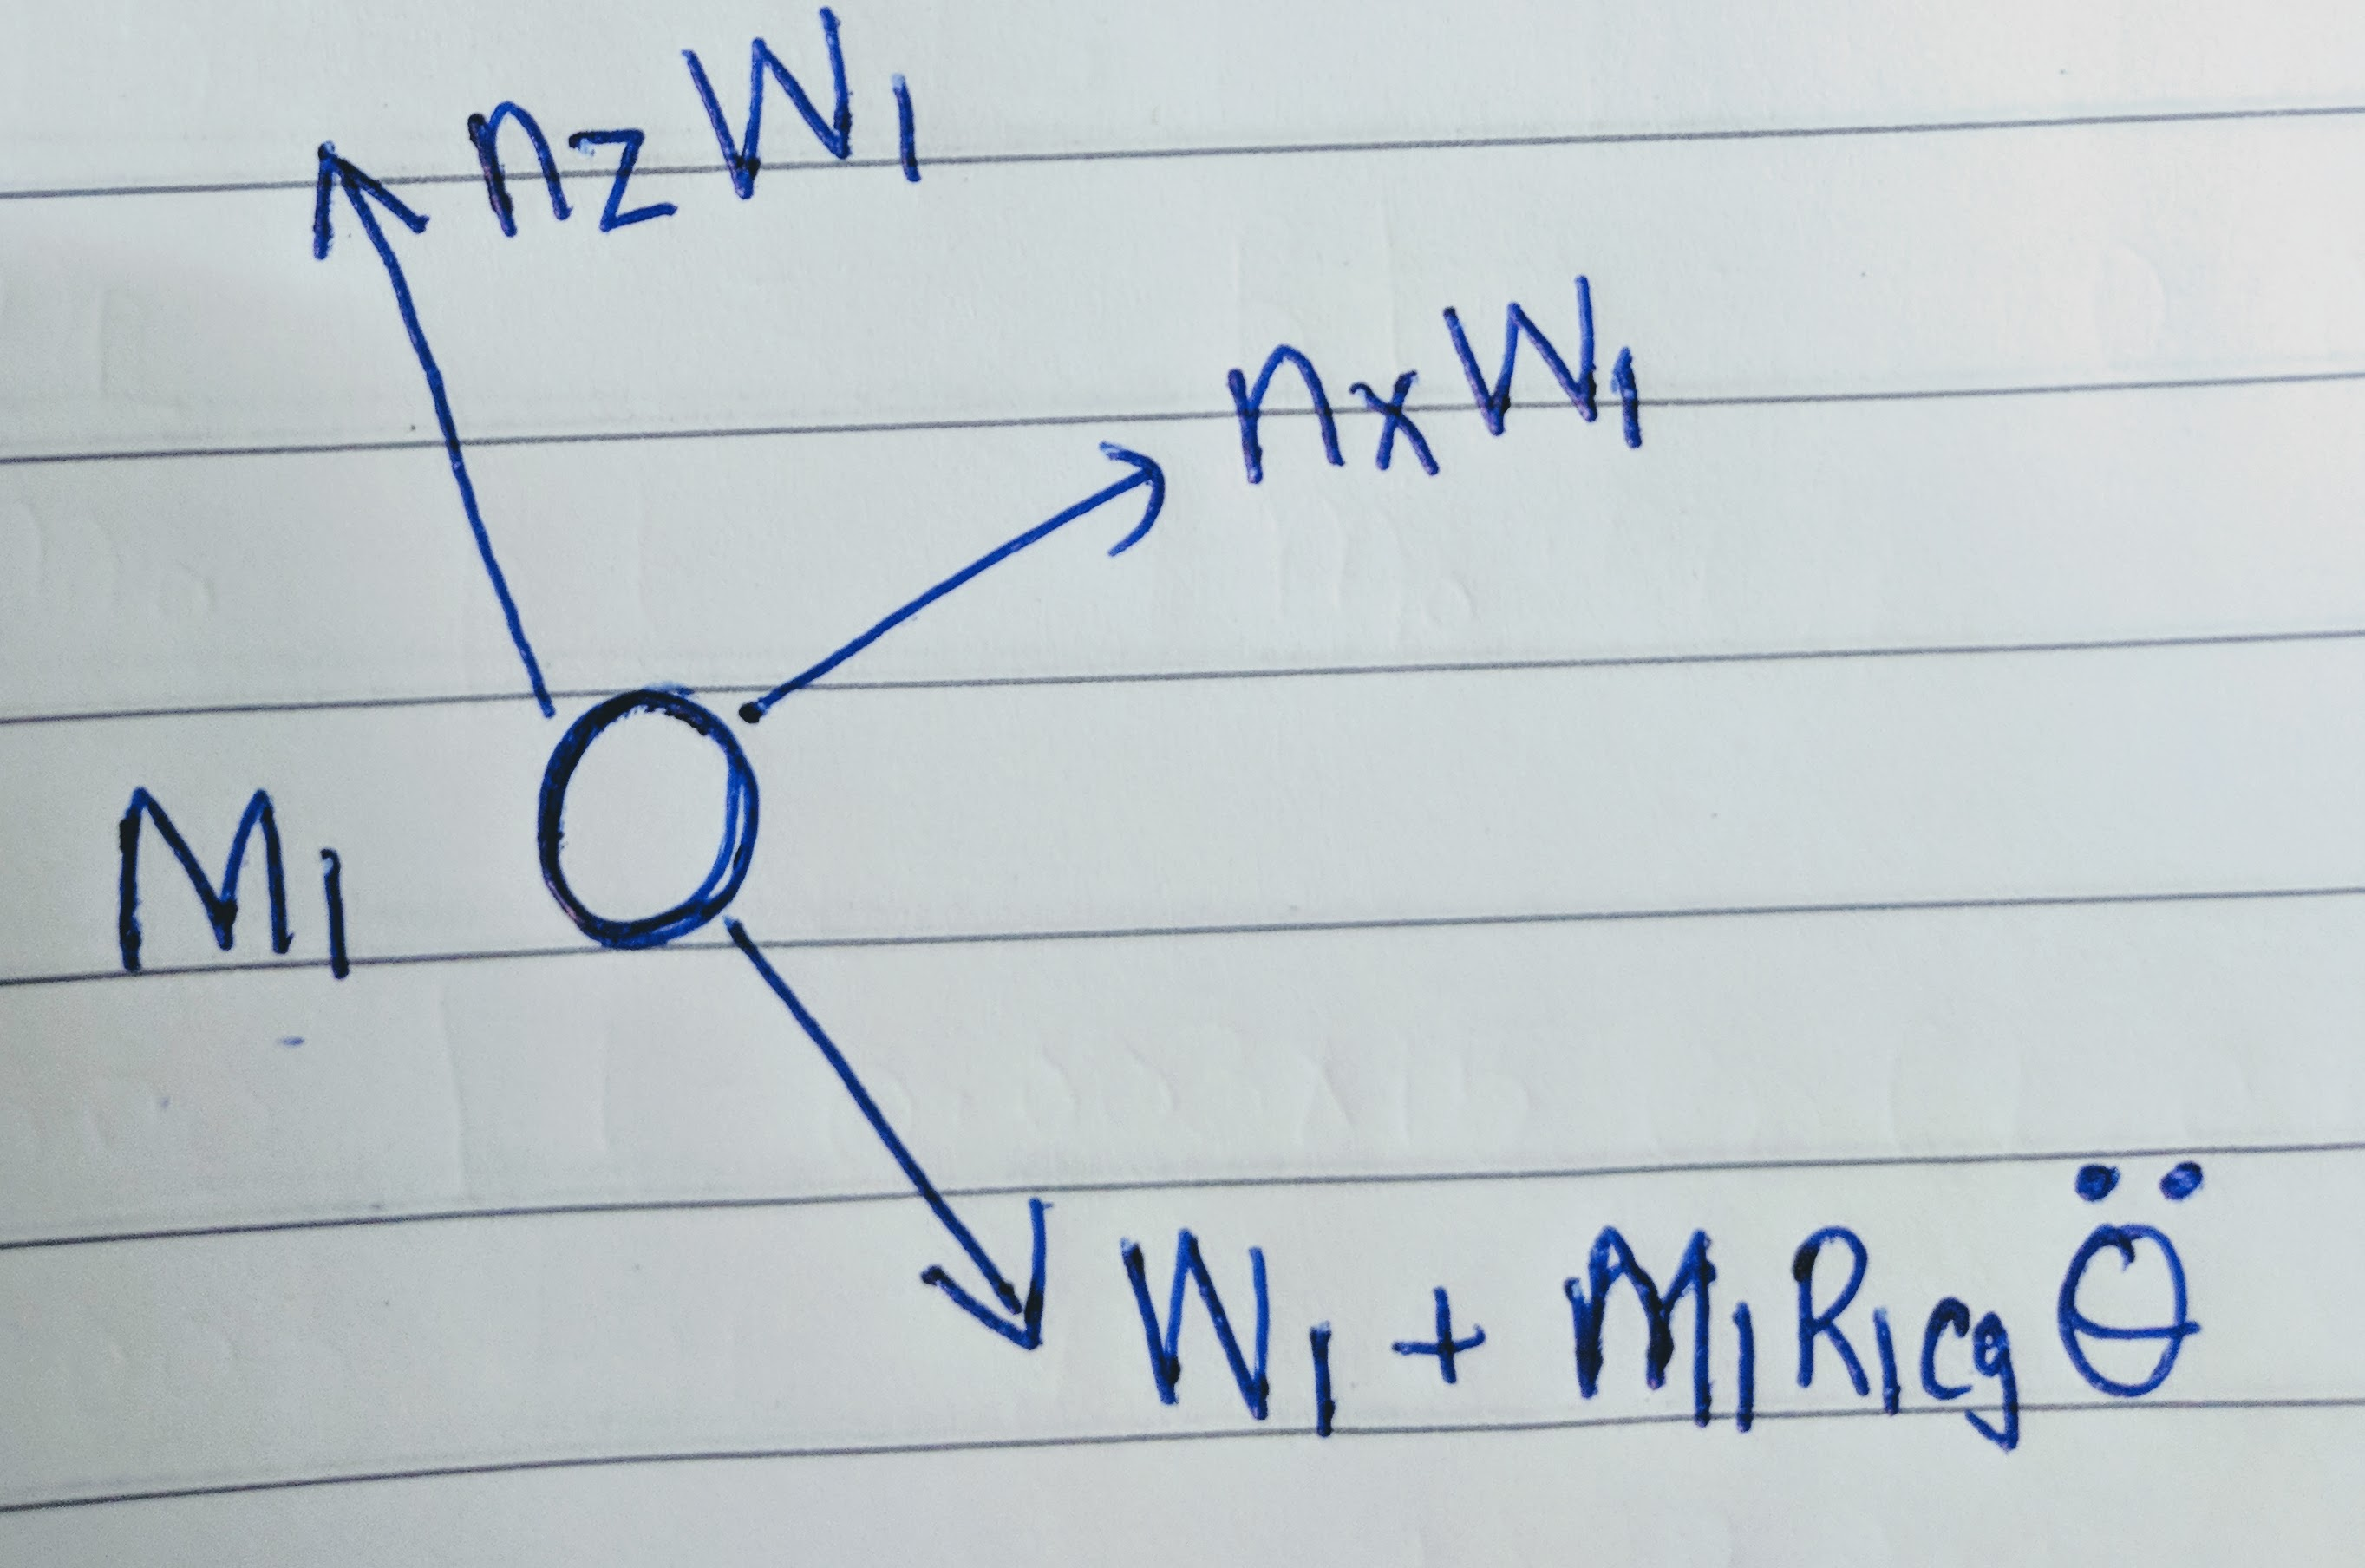
\includegraphics[scale=0.05]{m1.jpg}


\noindent In $x$ direction:\\

$\implies n_xW_1= 1000 N $\\

\noindent In $z$ direction: \\

\noindent $n_zW_1= 3.5 \times 50 \times 10\ N$\\
$\implies n_zW_1 = 1750\ N$\\

\noindent $M_1\ddot{\theta}R_{1cg}=50 \times 0.36 \times 0.75\ N $\\
$\implies M_1\ddot{\theta}R_{1cg}= 13.5\ N $\\

\noindent Apparent Weight in $z$ direction = net force in z direction. So : \\
$W_{A1,z}=\sum F_z = (n_zW_1-W_1- M_1\ddot{\theta}R_{1cg})\ N$\\
$W_{A1,z}= 1750- 13.5- 500\ N$\\
$\implies W_{A1,z}= 1236.5\ N$\\

\noindent Resultant apparent weight: \\
$W_{A1}= \sqrt{F_{net,x}^2+ F_{net,z}^2}\ N$\\
$\implies W_{A1}= \sqrt{1236.5^2+ 1000^2}\ N$\\
$\implies W_{A1}= 1590.26\ N$\\

\noindent \underline{Analyzing Mass $M_2$}:\\

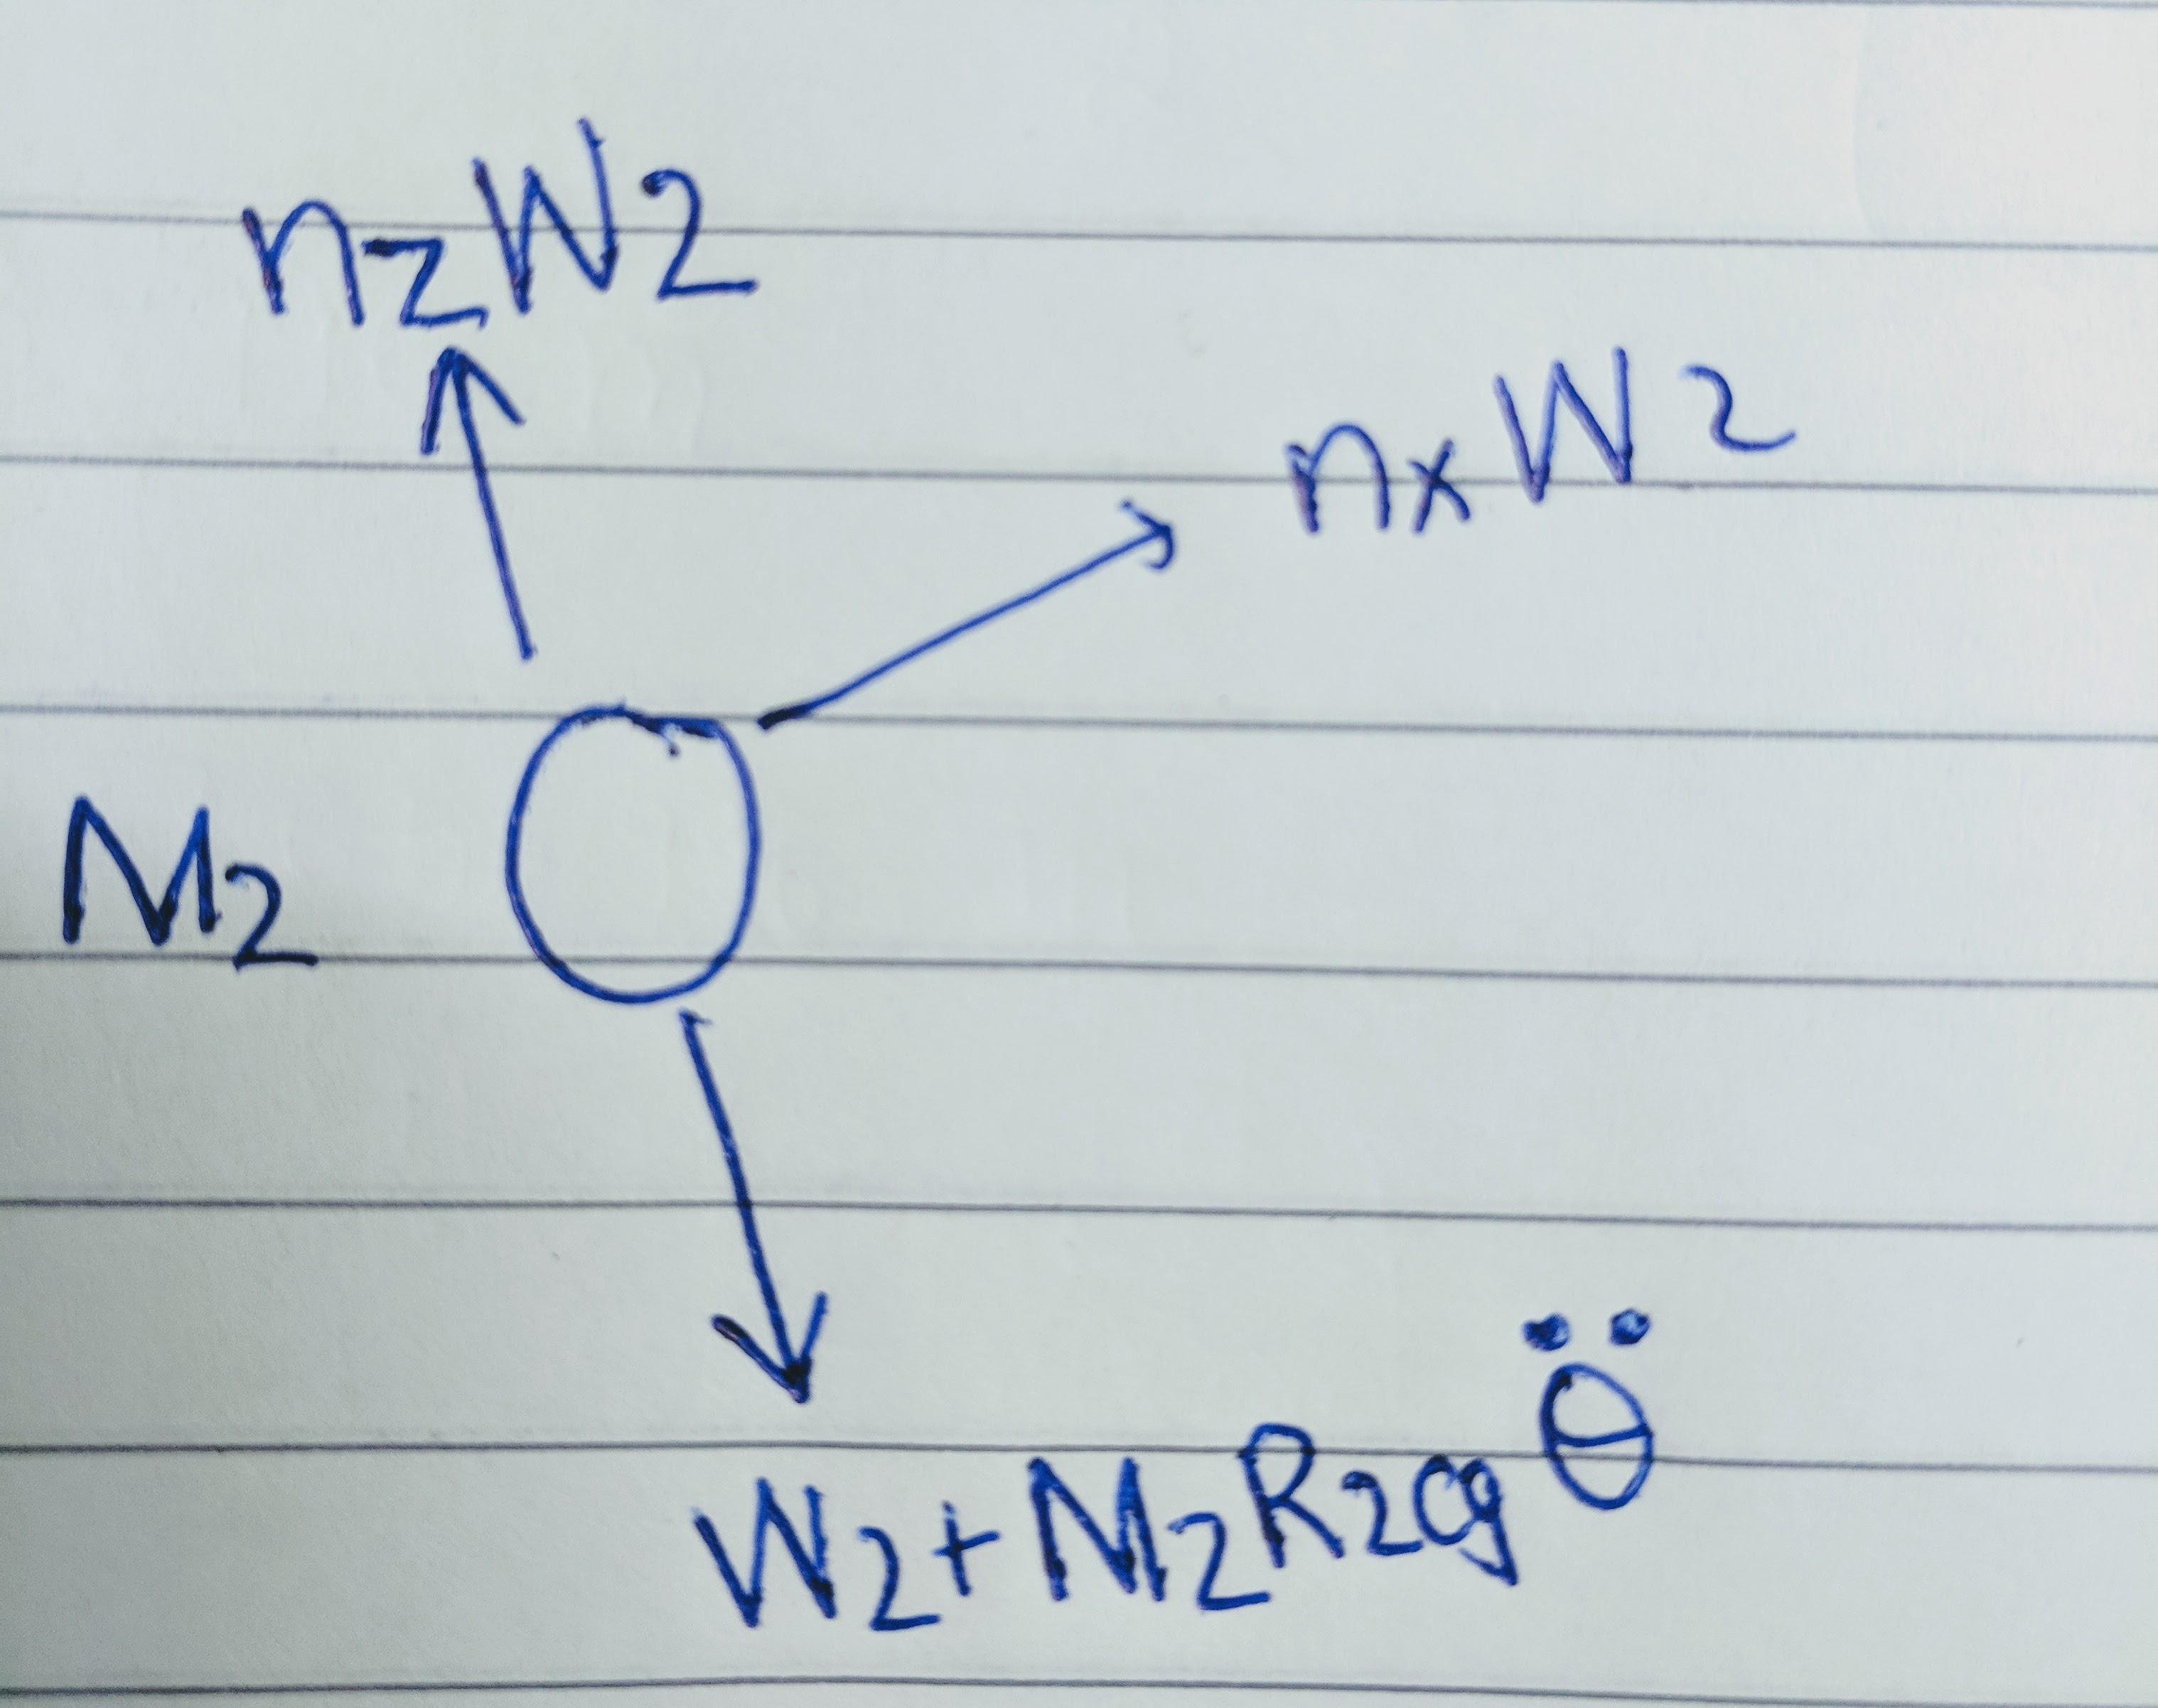
\includegraphics[scale=0.05]{m2.jpg}

\noindent In $x$ direction:\\

\noindent $n_xW_2 = 2 \times 200 \times 10\ N$\\
$\implies n_xW_2= 4000 N $\\

\noindent In $z$ direction: \\

\noindent $n_zW_2= 3.5 \times 200 \times 10\ N$\\
$\implies n_zW_2 = 7000\ N$\\

\noindent $M_2\ddot{\theta}R_{2cg}=200 \times 0.16 \times 0.75\ N $\\
$\implies M_2\ddot{\theta}R_{2cg}= 24\ N $\\

\noindent Apparent Weight in $z$ direction = net force in z direction. So : \\
$W_{A2,z}=\sum F_z = (n_zW_2-W_2- M_2\ddot{\theta}R_{2cg})\ N$\\
$W_{A2,z}= 7000-24-2000 \ N$\\
$\implies W_{A2,z}= 4976\ N$\\

\noindent Resultant apparent weight: \\
$W_{A2}= \sqrt{F_{net,x}^2+ F_{net,z}^2}\ N$\\
$\implies W_{A2}= \sqrt{4976^2+ 4000^2}\ N$\\
$\implies W_{A2}= 6384.40\ N$\\

\noindent \underline{Analyzing Mass $M_3$}:\\

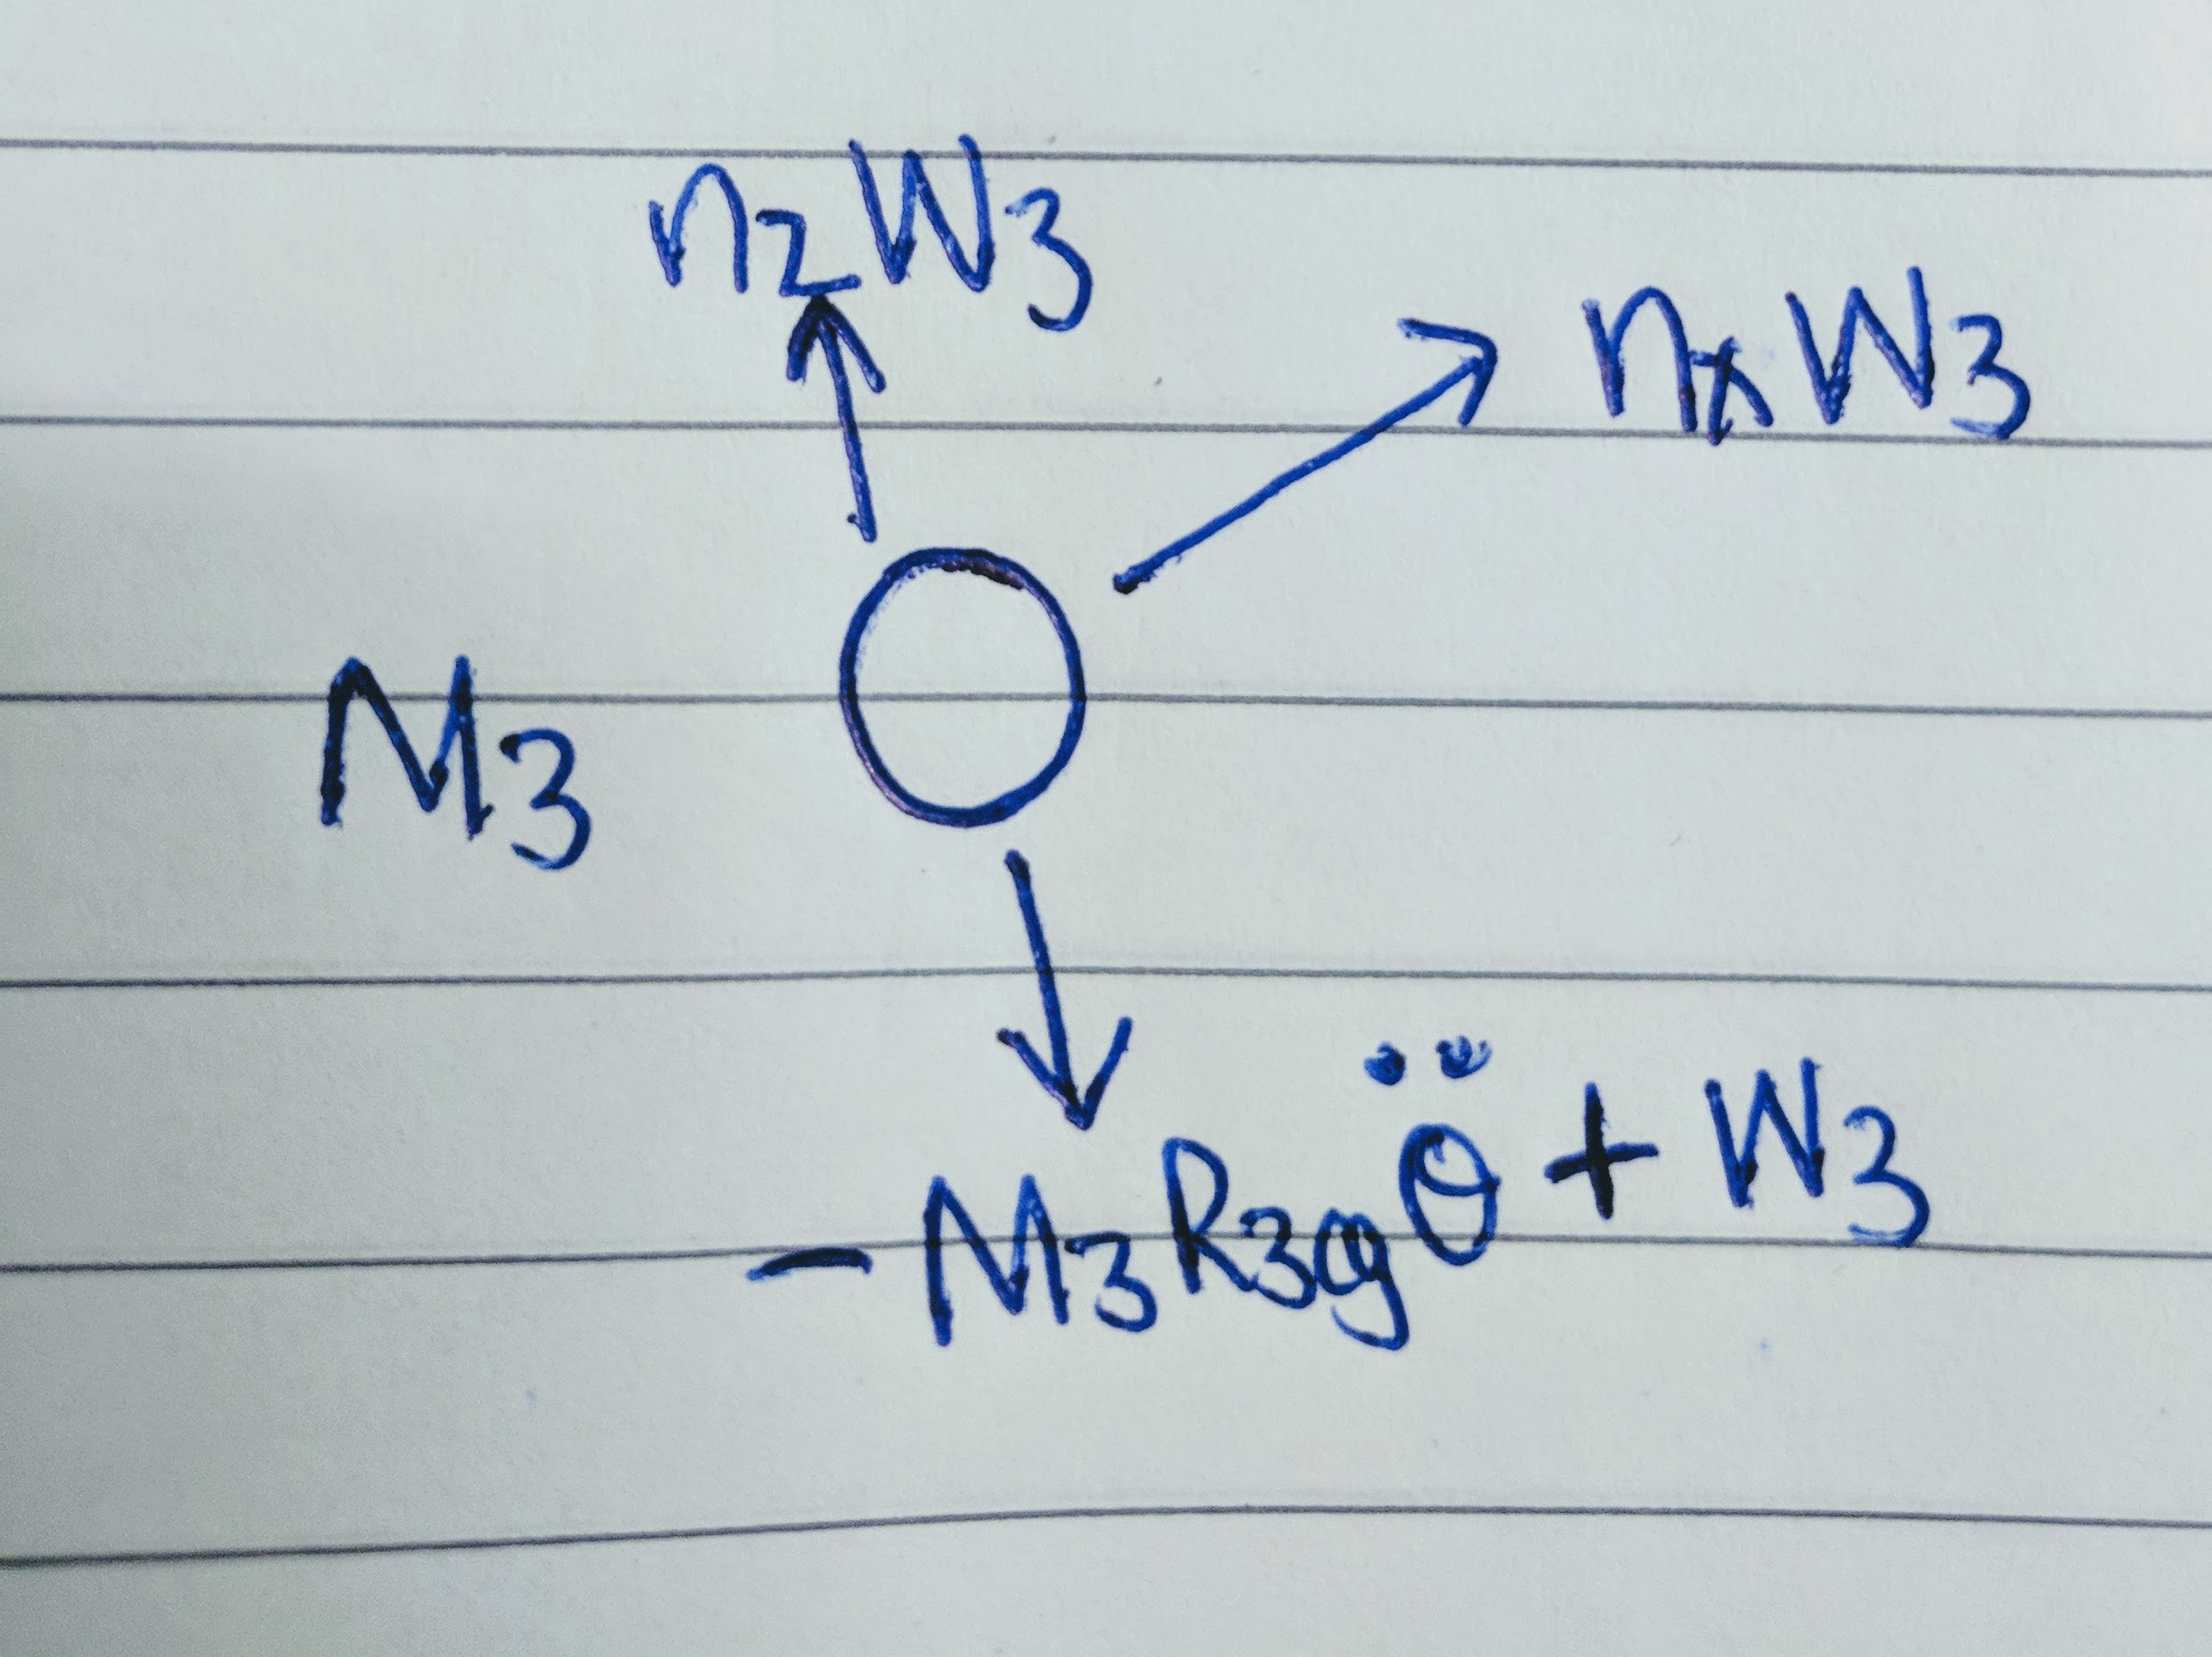
\includegraphics[scale=0.05]{m3.jpg}

\noindent In $x$ direction:\\

\noindent $n_xW_3 = 2 \times 100 \times 10\ N$\\
$\implies n_xW_3= 2000 N $\\

\noindent In $z$ direction: \\

\noindent $n_zW_3= 3.5 \times 100 \times 10\ N$\\
$\implies n_zW_3 = 3500\ N$\\

\noindent $M_3\ddot{\theta}R_{3cg}=100 \times 0.04 \times 0.75\ N $\\
$\implies M_3\ddot{\theta}R_{3cg}= 3\ N $\\

\noindent Apparent Weight in $z$ direction = net force in z direction. So : \\
$W_{A3,z}=\sum F_z = (n_zW_3-W_3+ M_3\ddot{\theta}R_{3cg})\ N$\\
$W_{A3,z}= 3500-1000+3 \ N$\\
$\implies W_{A3,z}= 2503\ N$\\

\noindent Resultant apparent weight: \\
$W_{A3}= \sqrt{F_{net,x}^2+ F_{net,z}^2}\ N$\\
$\implies W_{A3}= \sqrt{2503^2+ 2000^2}\ N$\\
$\implies W_{A3}= 3203.91\ N$\\

\noindent \underline{Analyzing Mass $M_4$}:\\

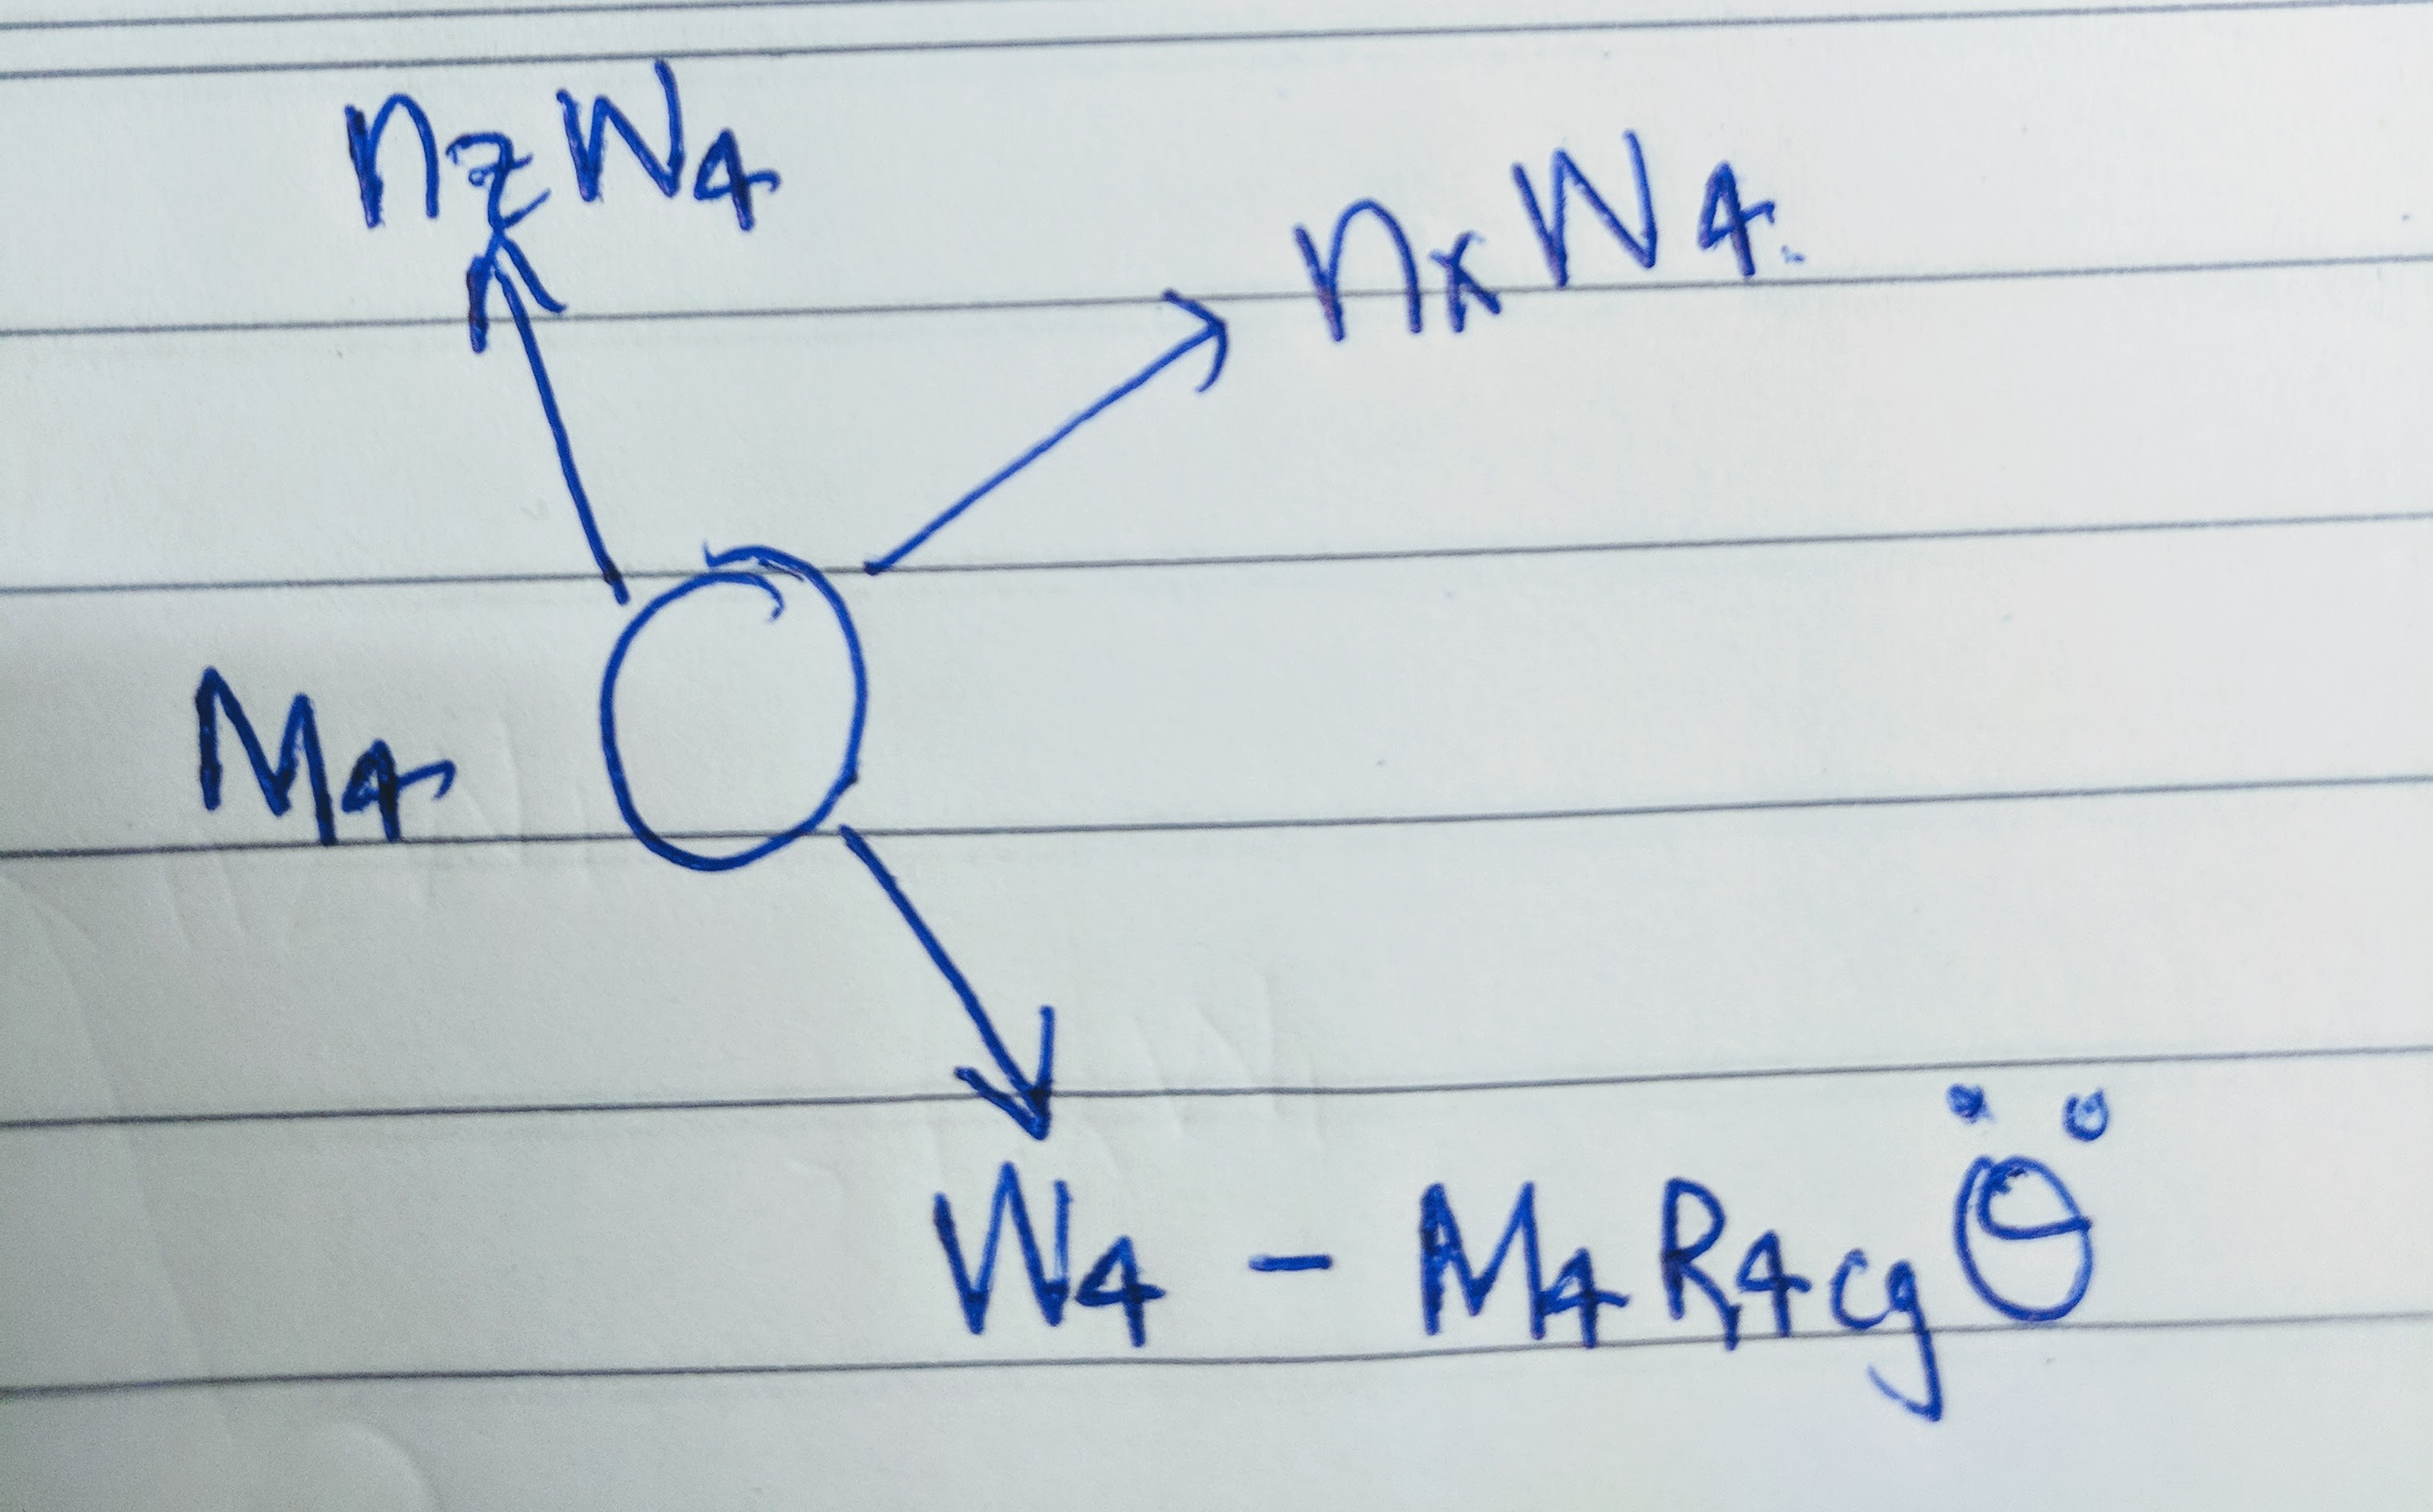
\includegraphics[scale=0.05]{m4.jpg}

\noindent In $x$ direction:\\

\noindent $n_xW_4 = 2 \times 100 \times 10\ N$\\
$\implies n_xW_4= 2000 N $\\

\noindent In $z$ direction: \\

\noindent $n_zW_4= 3.5 \times 100 \times 10\ N$\\
$\implies n_zW_4 = 3500\ N$\\

\noindent $M_4\ddot{\theta}R_{4cg}=100 \times 0.24 \times 0.75\ N $\\
$\implies M_4\ddot{\theta}R_{4cg}= 18\ N $\\

\noindent Apparent Weight in $z$ direction = net force in z direction. So : \\
$W_{A4,z}=\sum F_z = (n_zW_4-W_4+ M_4\ddot{\theta}R_{4cg})\ N$\\
$W_{A4,z}= 3500-1000+18 \ N$\\
$\implies W_{A4,z}= 2518\ N$\\

\noindent Resultant apparent weight: \\
$W_{A4}= \sqrt{F_{net,x}^2+ F_{net,z}^2}\ N$\\
$\implies W_{A4}= \sqrt{2518^2+ 2000^2}\ N$\\
$\implies W_{A4}= 3215.64\ N$\\

\noindent \underline{Analyzing Mass $M_5$}:\\

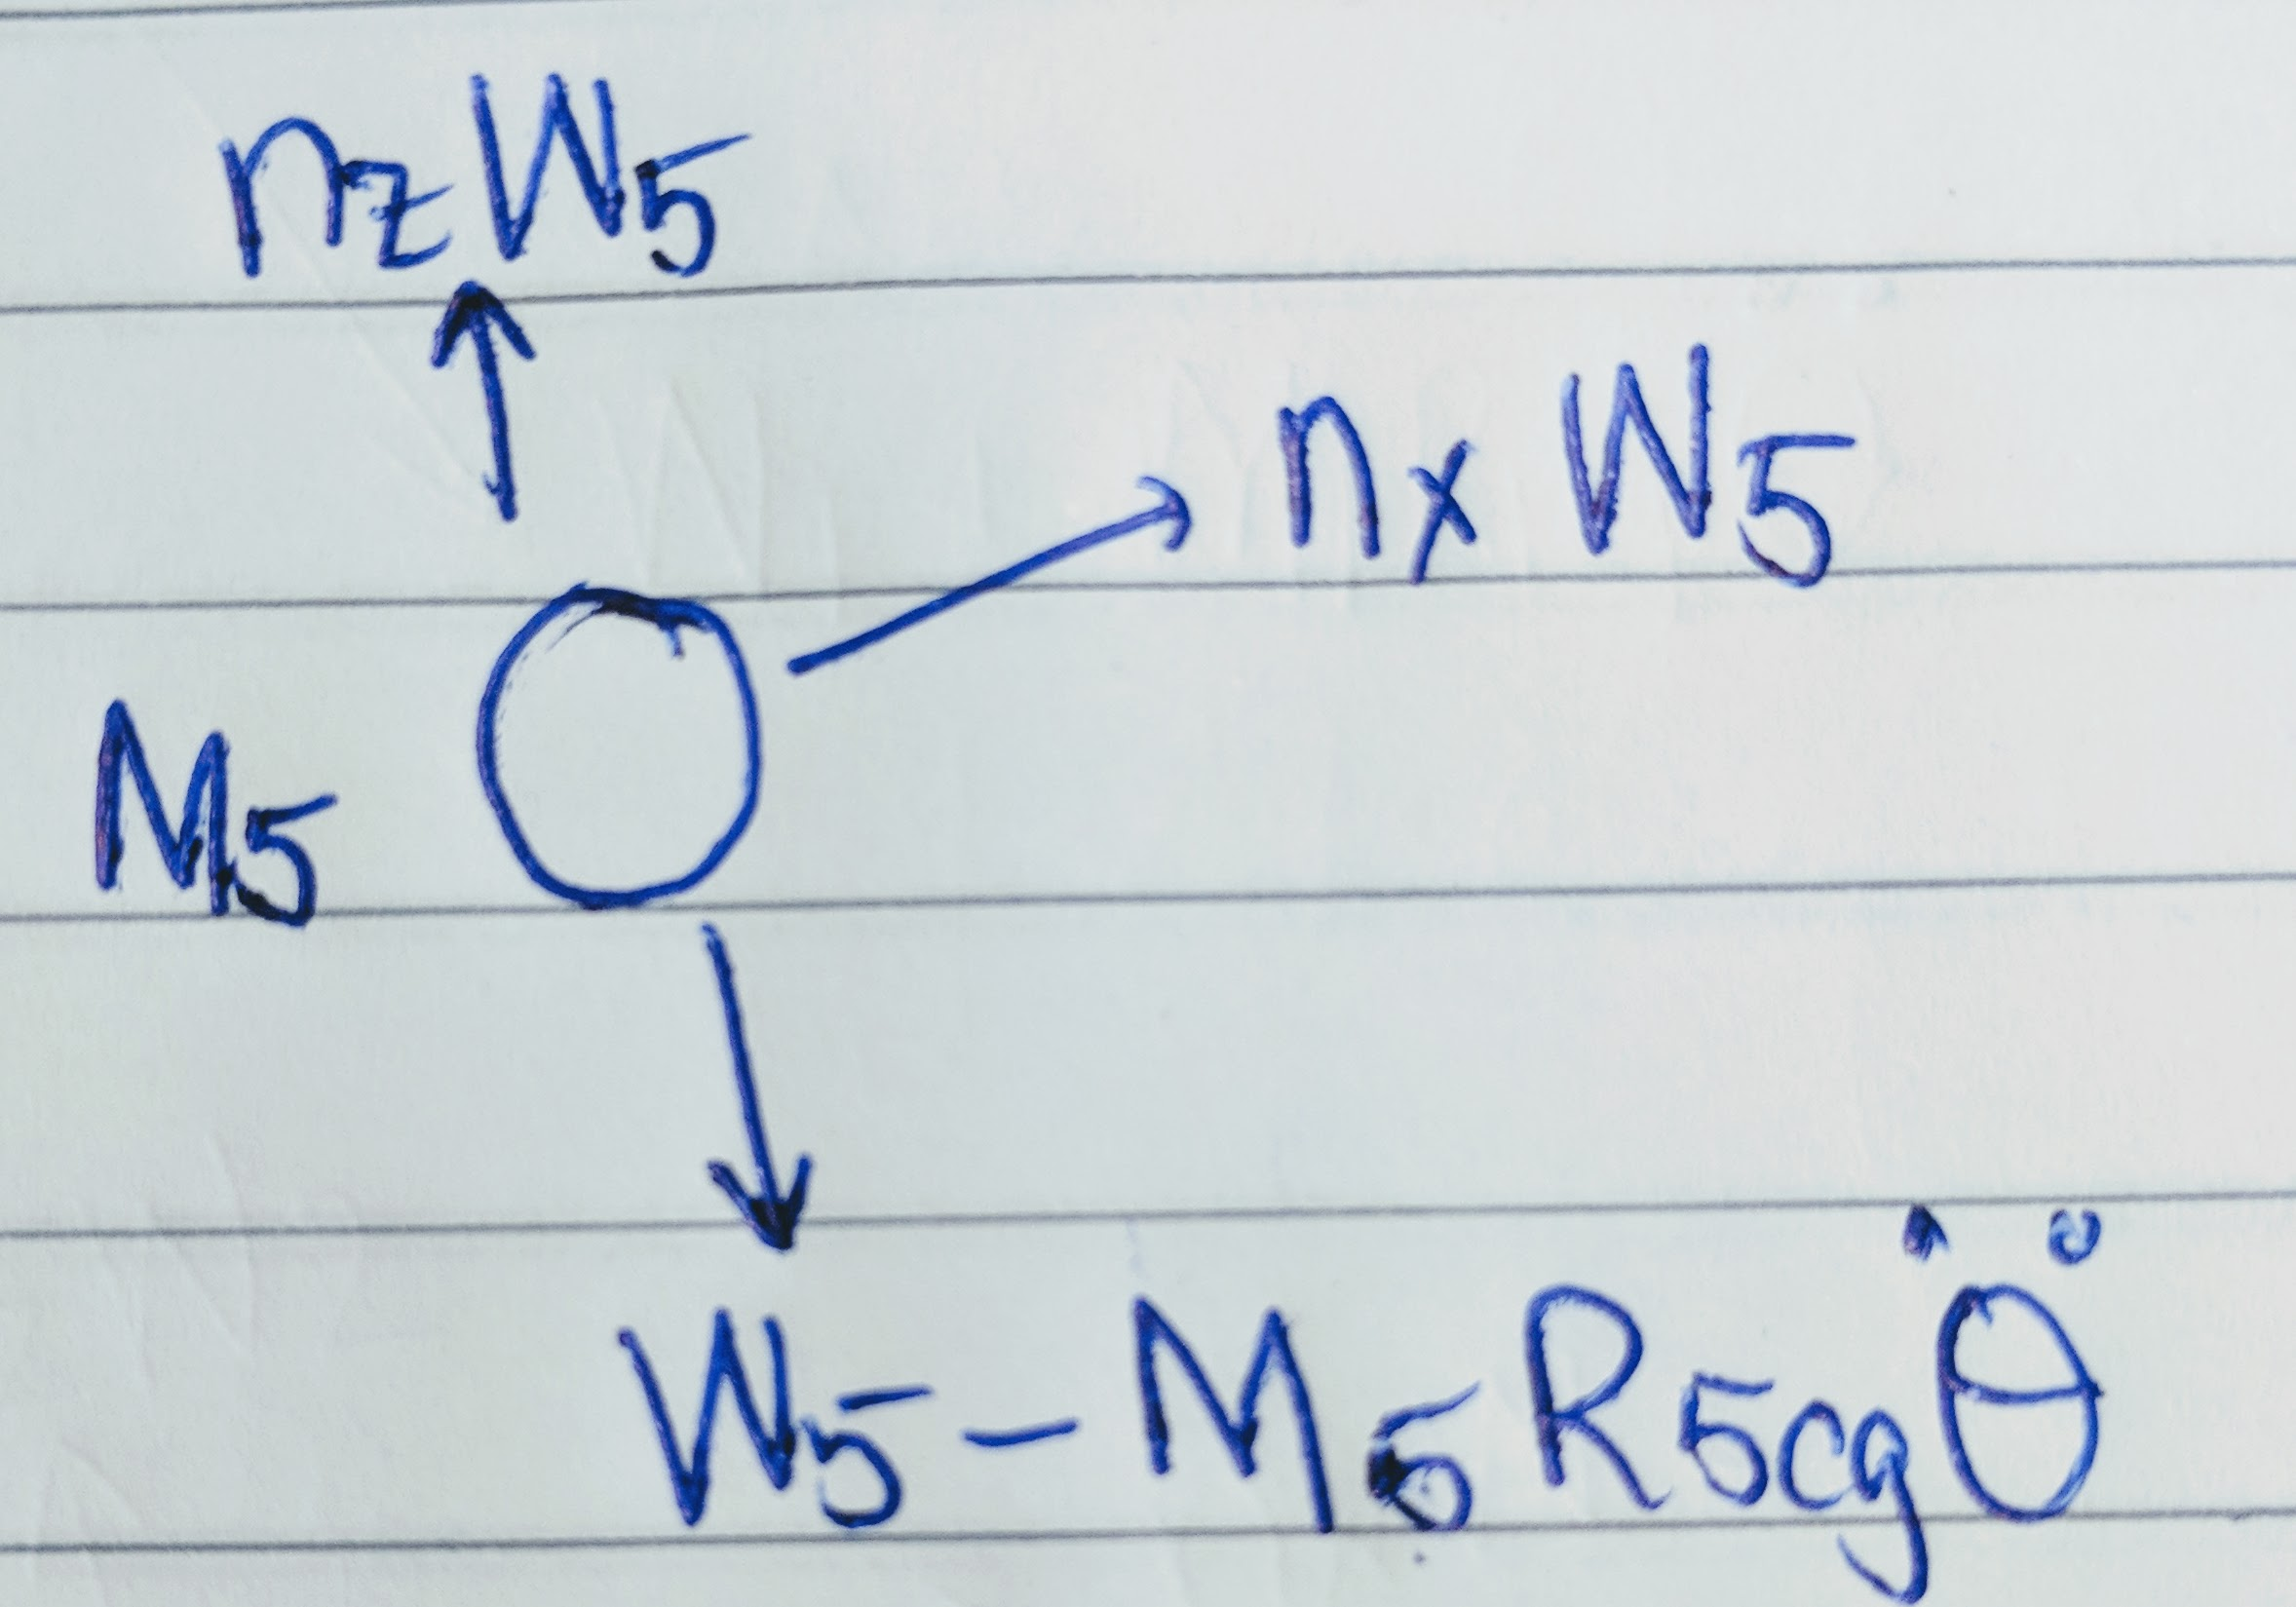
\includegraphics[scale=0.05]{m5.jpg}

\noindent In $x$ direction:\\

\noindent $n_xW_5 = 2 \times 50 \times 10\ N$\\
$\implies n_xW_5= 1000 N $\\

\noindent In $z$ direction: \\

\noindent $n_zW_5= 3.5 \times 50 \times 10\ N$\\
$\implies n_zW_5 = 1750\ N$\\

\noindent $M_5\ddot{\theta}R_{5cg}=50 \times 0.44 \times 0.75\ N $\\
$\implies M_5\ddot{\theta}R_{5cg}= 16.5\ N $\\

\noindent Apparent Weight in $z$ direction = net force in z direction. So : \\
$W_{A5,z}=\sum F_z = (n_zW_5-W_5+ M_5\ddot{\theta}R_{5cg})\ N$\\
$W_{A5,z}= 1750-500+16.5 \ N$\\
$\implies W_{A5,z}= 1266.5\ N$\\

%\newpage
\noindent Resultant apparent weight: \\
$W_{A5}= \sqrt{F_{net,x}^2+ F_{net,z}^2}\ N$\\
$\implies W_{A5}= \sqrt{1266.5^2+ 1000^2}\ N$\\
$\implies W_{A5}= 1613.69\ N$\\

\noindent \underline{Finding bending moment about centre of gravity} (counter-clockwise moment is cosidered positive):\\

\noindent $M= \sum_{i=1}^5F_{zi}R_{i,cg}= \sum_{i=1}^5W_{Ai,z}R_{i,cg}$\\
$ M=-(1236.5)(0.36)-(4976)(0.16)+(2503)(0.04)+(2518)(0.24)+(1266.5)(0.44)$ \\
$M=20.4\ Nm$\\
\bigbreak
\begin{center}
\title{\textbf{\LARGE \underline{THE END}}}
\end{center}
\end{document}

